\section{Scanner and Parser Generators}
\begin{frame}{Scanner and Parser Generators}
  \begin{itemize}
    \item Parser overview
    \item Parser generators
    \item Lexer
    \item CFG
  \end{itemize}
\end{frame}

\begin{frame}{Parser overview}
  Automate the generation of lexer and parser.
\begin{figure}[ht]
\centering
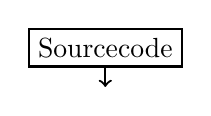
\begin{tikzpicture}
  \draw [thick, ->] (0,0.3) -- (0,0);
  \node [rectangle, draw, thick,fill=white!20] at (0,0.5) {Sourcecode};
\end{tikzpicture}

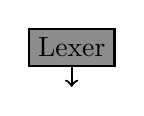
\begin{tikzpicture}
  \draw [thick, ->] (0,0.3) -- (0,0);
  \node [rectangle, draw, thick,fill=gray!90] at (0,0.5) {Lexer};
\end{tikzpicture}

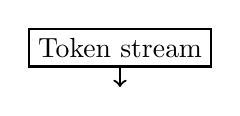
\begin{tikzpicture}
  \draw [thick, ->] (0,0.3) -- (0,0);
  \node [rectangle, draw, thick,fill=white!20] at (0,0.5) {Token stream};
\end{tikzpicture}

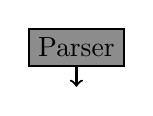
\begin{tikzpicture}
  \draw [thick, ->] (0,0.3) -- (0,0);
  \node [rectangle, draw, thick,fill=gray!90] at (0,0.5) {Parser};
\end{tikzpicture}

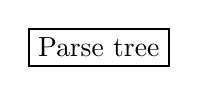
\begin{tikzpicture}
  \node [rectangle, draw, thick,fill=white!20] at (0,0.5) {Parse tree};
\end{tikzpicture}
\end{figure}
\end{frame}

\subsection{Parser Generators}
\begin{frame}{Parser Generators}
  \framesubtitle{Different parser generators}
  \begin{itemize}
    \item SableCC
    \item JavaCup
    \item ANTLR
    \item Coco/R
    \item Yacc
    \item And many mores.
  \end{itemize}
\end{frame}

\begin{frame}{SableCC}
  \begin{itemize}
    \item OO Java LALR(1) Parser generator
    \begin{itemize}
      \item also exsist for other languages
    \end{itemize}
    \item Input
    \begin{itemize}
      \item Token rules
      \item Grammar productions
    \end{itemize}
    \item Output
    \begin{itemize}
      \item Lexer
      \item Parser
      \item AST classes
      \item AST walkers
    \end{itemize}
  \end{itemize}
\end{frame}

\begin{frame}{JavaCup}
  \begin{itemize}
    \item Java LALR(1) parser generator
    \begin{itemize}
      \item Does not include lexer generator
    \end{itemize}
    \item Input
    \begin{itemize}
      \item Grammar productions
      \item Optional action code
    \end{itemize}
    \item Output
    \begin{itemize}
      \item Parser
    \end{itemize}
  \end{itemize}
\end{frame}

\begin{frame}{ANTLR}
 \begin{itemize}
    \item Java LL(*) parser generator
    \begin{itemize}
      \item Can be used with ANTLRWorks IDE
    \end{itemize}
    \item Input
    \begin{itemize}
      \item Token rules
      \item Grammar productions
    \end{itemize}
    \item Output
    \begin{itemize}
      \item Lexer
      \item Parser
      \item Error Reporting
    \end{itemize}
  \end{itemize}
\end{frame}


\subsection{Tokens and Lexer}
\begin{frame}[fragile]{Tokens}
\framesubtitle{Generating a lexer}
 Generates tokens from sourcecode

\begin{lstlisting}[caption=Example af lexer rules in GAMBL.,frame=tlrb, basicstyle=\tiny, numbers=none]
INT: 'int' | 'int16' | 'int32' | 'int64' ;
INTNUM: '0' | SIGN? [1-9][0-9]* ;
\end{lstlisting}
\end{frame}


\subsection{CFG}
\begin{frame}[fragile]{GAMBL's CFG}
 \begin{lstlisting}[caption=Grammar rules for the expression production in GAMBL.,frame=tlrb, basicstyle=\tiny, numbers=none]
expression
    : expression '^' expression                         #powerExpr
    | expression ( '*' | '/' | '%' | '#' ) expression   #mulExpr
    | expression ( '+' | '-' ) expression               #addExpr
    | '(' expression ')'                                #parenExpr
    | value                                             #valueExpr
    | ID postUnaryOperator                              #postIDExpr
    ;
\end{lstlisting}
\end{frame}



